\documentclass[a4paper,11pt]{article}
\usepackage[left=2.5cm,right=2.5cm]{geometry}
\usepackage{graphicx}
\usepackage{float}
\usepackage{listings}
\usepackage{color}
\usepackage{amsmath}
\usepackage{hyperref}
\hypersetup{colorlinks=true,linkcolor=blue,urlcolor=blue}
  
\definecolor{codegreen}{rgb}{0,0.6,0}
\definecolor{codegray}{rgb}{0.5,0.5,0.5}
\definecolor{codepurple}{rgb}{0.58,0,0.82}
\definecolor{backcolour}{rgb}{0.95,0.95,0.92}
 
\lstdefinestyle{mystyle}{
    backgroundcolor=\color{backcolour},   
    commentstyle=\color{codegreen},
    keywordstyle=\color{magenta},
    numberstyle=\tiny\color{codegray},
    stringstyle=\color{codepurple},
    basicstyle=\footnotesize,
    breakatwhitespace=false,         
    breaklines=true,                 
    captionpos=t,                    
    keepspaces=true,                 
    numbers=left,                    
    numbersep=5pt,                  
    showspaces=false,                
    showstringspaces=false,
    showtabs=false,                  
    tabsize=2
}
 
\lstset{style=mystyle}
\graphicspath{{./imgs/}}
\pagenumbering{gobble}
\allowdisplaybreaks

\begin{document}

 \begin{center}
  \large{\textbf{CSE578 Computer Vision}}\\
  \Large{\textbf{Assignment 1 : Camera Calibration}}\\
  \vspace{1em}
  Karnik Ram\\
  2018701007
 \end{center}
 
 \section{Direct Linear Transform}
 
 The Direct Linear Transform (DLT) algorithm is used to estimate the camera matrix (11 dof) from a set of atleast 6 2D-3D point corespondences. The algorithm is based on solving the system of linear equations $x = PX$, which is then simply rearranged to form a system $Mp = 0$. $p$ is a $12 \times 1$ vector and $M$ is a $2N * 12$ matrix where $N$ is the number of correspondences. The solution $p$ is obtained using SVD which is then rearranged to form back the matrix $P$. $P$ is then decomposed into $K,R,C$ using RQ decomposition.
 
  \subsection{Code/Algorithm}
  The following is a snippet from Listing 2 (Section 11) which implements DLT.
  \begin{lstlisting}[language=C++]
  
 void Calibrator::calibrateByDlt(const std::vector<int> &sample_indices)
{
	if(sample_indices.size() < 6)
	{
		std::cout << "Cannot run DLT! Require at least 6 correspondences.\n";
		return;
	}

	Eigen::MatrixXf X_samples(sample_indices.size(),4);
	Eigen::MatrixXf x_samples(sample_indices.size(),3);

	if(sample_indices.size() == X.rows())
	{
		X_samples = X;
		x_samples = x;
	}

	else
	{	int j = 0;	
		for (int i : sample_indices)
		{
			X_samples.row(j) = X.row(i);
			x_samples.row(j++) = x.row(i);
		}
	}

	Eigen::ArrayXf p(12);
	Eigen::MatrixXf M(2*x_samples.rows(),12);

	// Build M
	for(int i = 0,j=0; i < M.rows(); i+=2,j++)
	{
		M.row(i) << X_samples.row(j) * -1, Eigen::MatrixXf::Zero(1,4), X_samples.row(j) * x_samples(j,0);
		M.row(i+1) << Eigen::MatrixXf::Zero(1,4), X_samples.row(j) * -1, X_samples.row(j) * x_samples(j,1);
	}

	// Estimate p
	Eigen::JacobiSVD<Eigen::MatrixXf> svd(M,Eigen::ComputeFullU | Eigen::ComputeFullV);
	Eigen::MatrixXf V;
	V = svd.matrixV();
	p = V.col(V.cols()-1);

	// Build P
 	P.resize(3,4);
	P.row(0) = p.segment(0,4);
	P.row(1) = p.segment(4,4);
	P.row(2) = p.segment(8,4);
	std::cout << "P:\n" << P << std::endl;
	std::cout << "Average reprojection error:\n" << calcAvgReprojectionError() << std::endl;
} 
  \end{lstlisting}

  \vspace{2em}
  
 \section{DLT with RANSAC}
 Random sample consensus (RANSAC) is a robust estimation algorithm. The idea is to determine a set of inliers from the set of correspondences, which are then used to estimate the calibration parameters. This is done by repeatedly sampling minimal sets (6 correspondences) and estimating the model, and then choosing the model which is supported by the maximum number of inliers. Inliers are determined using user specified distance and ratio thresholds.
  \subsection{Code/Algorithm}
  The following is a snippet from Listing 2 (Section 11) which implements DLT inside a RANSAC scheme.
  \begin{lstlisting}[language=C++]
  
 void Calibrator::calibrateByDltRansac(const float &dist_threshold, const float &inlier_ratio, std::vector<int> &inlier_indices)
{	
	std::cout << "Running RANSAC...." << std::endl;
	std::vector<int> largest_support;

	for(int n = 0; n < 500; n++)
	{
		std::cout << "\n\nIteration #" << n+1 << std::endl;
		std::vector<int> sample_indices = utils::generateRandomVector(0,X.rows()-1,6);
		calibrateByDlt(sample_indices);
	
		for(int i = 0; i < X.rows(); i++)
		{
			float dist = calcReprojectionError(X.row(i),x.row(i));
			if(dist < dist_threshold)
				inlier_indices.push_back(i); 
		}

		if(inlier_indices.size() >= inlier_ratio * X.rows())
		{
			std::cout << "Found a model!\n" << "Number of inliers: " << inlier_indices.size() << std::endl;
			std::cout << "Inliers: ";
			for(int i : inlier_indices)
				std::cout << i << " ";

			std::cout << "\n";
			calibrateByDlt(inlier_indices);
			return;
		}
	
		else
		{
			if(largest_support.size() <= inlier_indices.size())
				largest_support = inlier_indices;

			inlier_indices.clear();
		}
	}

	if(largest_support.size() >= 6)
	{
		std::cout << "Could not find a model according to threshold!\nSo using largest inlier set instead." << std::endl;
		calibrateByDlt(largest_support);
		inlier_indices = largest_support;
		std::cout << "Number of inliers: " << inlier_indices.size() << std::endl;
		for(int i : inlier_indices)
			std::cout << i << " ";

		std::cout << "\n";
	}

	else
		std::cout << "Could not find a model!" << std::endl;
} 
  
  \end{lstlisting}
  
  \vspace{2em}
 
 \section{Results using the provided setup}
  
  The 2D and 3D points were measured manually from the provided images. The Z-axis of the world frame was taken to be pointing into the object to make it a right-handed coordinate frame for convenience. The estimated parameters were validated using the average reprojection error as a metric.
 \subsection*{DLT}
  \begin{align*}
  \text{Calibration matrix}
  &:
  \begin{pmatrix}
  12077.4 & -149.151 & 3008.17 \\
  0 & 12200.9 & 2970.19 \\
  0 & 0 & 1 \\
  \end{pmatrix}\\
  \text{Rotation matrix}
  &:
  \begin{pmatrix}
   -0.9780 & 0.0072 & 0.2084 \\
   -0.0916 & -0.9126 & -0.3983 \\
   0.1873 & -0.4086 & 0.8932 \\
  \end{pmatrix}\\
  \text{Camera center}
  &:
  \begin{pmatrix}
   -0.1435\\
   -0.0648\\
   -2.99\times10^{-5}\\
  \end{pmatrix}\\
  \text{Average reprojection error}
  &: 310.596\\
  \end{align*}
 
 \subsection*{DLT with RANSAC}
 
    \begin{align*}
  \text{Calibration matrix}
  &:
  \begin{pmatrix}
  12578 & -216.138 & 2778.59 \\
  0 & 12633.2 & 2080.56 \\
  0 & 0 & 1 \\
  \end{pmatrix}\\
  \text{Rotation matrix}
  &:
  \begin{pmatrix}
   -0.9745 & -0.0016 & 0.2242 \\
   -0.0762 & -0.9380 & -0.3380 \\
   0.2109 & -0.3465 & 0.9140 \\
  \end{pmatrix}\\
  \text{Camera center}
  &:
  \begin{pmatrix}
   -0.1447\\
   -0.0648\\
   -3.0195\times10^{-5}\\
  \end{pmatrix}\\
  \text{Average reprojection error}
  &: 447.887\\
    \text{Reprojection error threshold}&: 250\\
  \text{Inlier ratio threshold}&: 0.8\
  \end{align*}
  
  The thresholds for RANSAC were set by trial-and-error. The maximum number of iterations was set to $500$.
 
 \section{Undistortion}
 
 The radial and tangential distortion parameters were estimated using Matlab's \texttt{estimateCamera}-\texttt{Parameters} function. The checkerboard images were used for this purpose. Using these parameters, the image of the 3D object was undistorted using OpenCV's \texttt{undistort} function. I assumed the 3D object, and the checkerboard were both captured using the same camera.
 
 The following are the estimated distortion parameters:
 \begin{align*}
  \text{Radial}&: 0.2963, -2.999,  20.5691\\
  \text{Tangential}&: 0.0017, 0.0112\\
 \end{align*}
 
 The three radial distortion values correspond to $k_1, k_2, k_3$, and tangential to $p_1, p_2$. The distortion parameters are usually estimated by finding the straight line in the image, and then doing a search over the values of $p_1,p_2,k_1,k_2,k_3$ that minimizes the distance between the midpoint of these lines and the average of their endpoints.
 \begin{align*}
  x_{\text{distortion}} &= x + (2p_1xy + p_2(r^2 + 2x^2))\\
  y_{\text{distortion}} &= x + (2p_2xy + p_1(r^2 + 2y^2))\\
  \\
  x_{\text{distortion}} &= x(1 + k_1r^2 + k_2r^4 + k_3r^6)\\
  y_{\text{distortion}} &= x(1 + k_1r^2 + k_2r^4 + k_3r^6)
 \end{align*}
 
 The following are the estimated camera parameters after undistorting the 3D calibration object image:
 
   \begin{figure}[H]
      \centering
      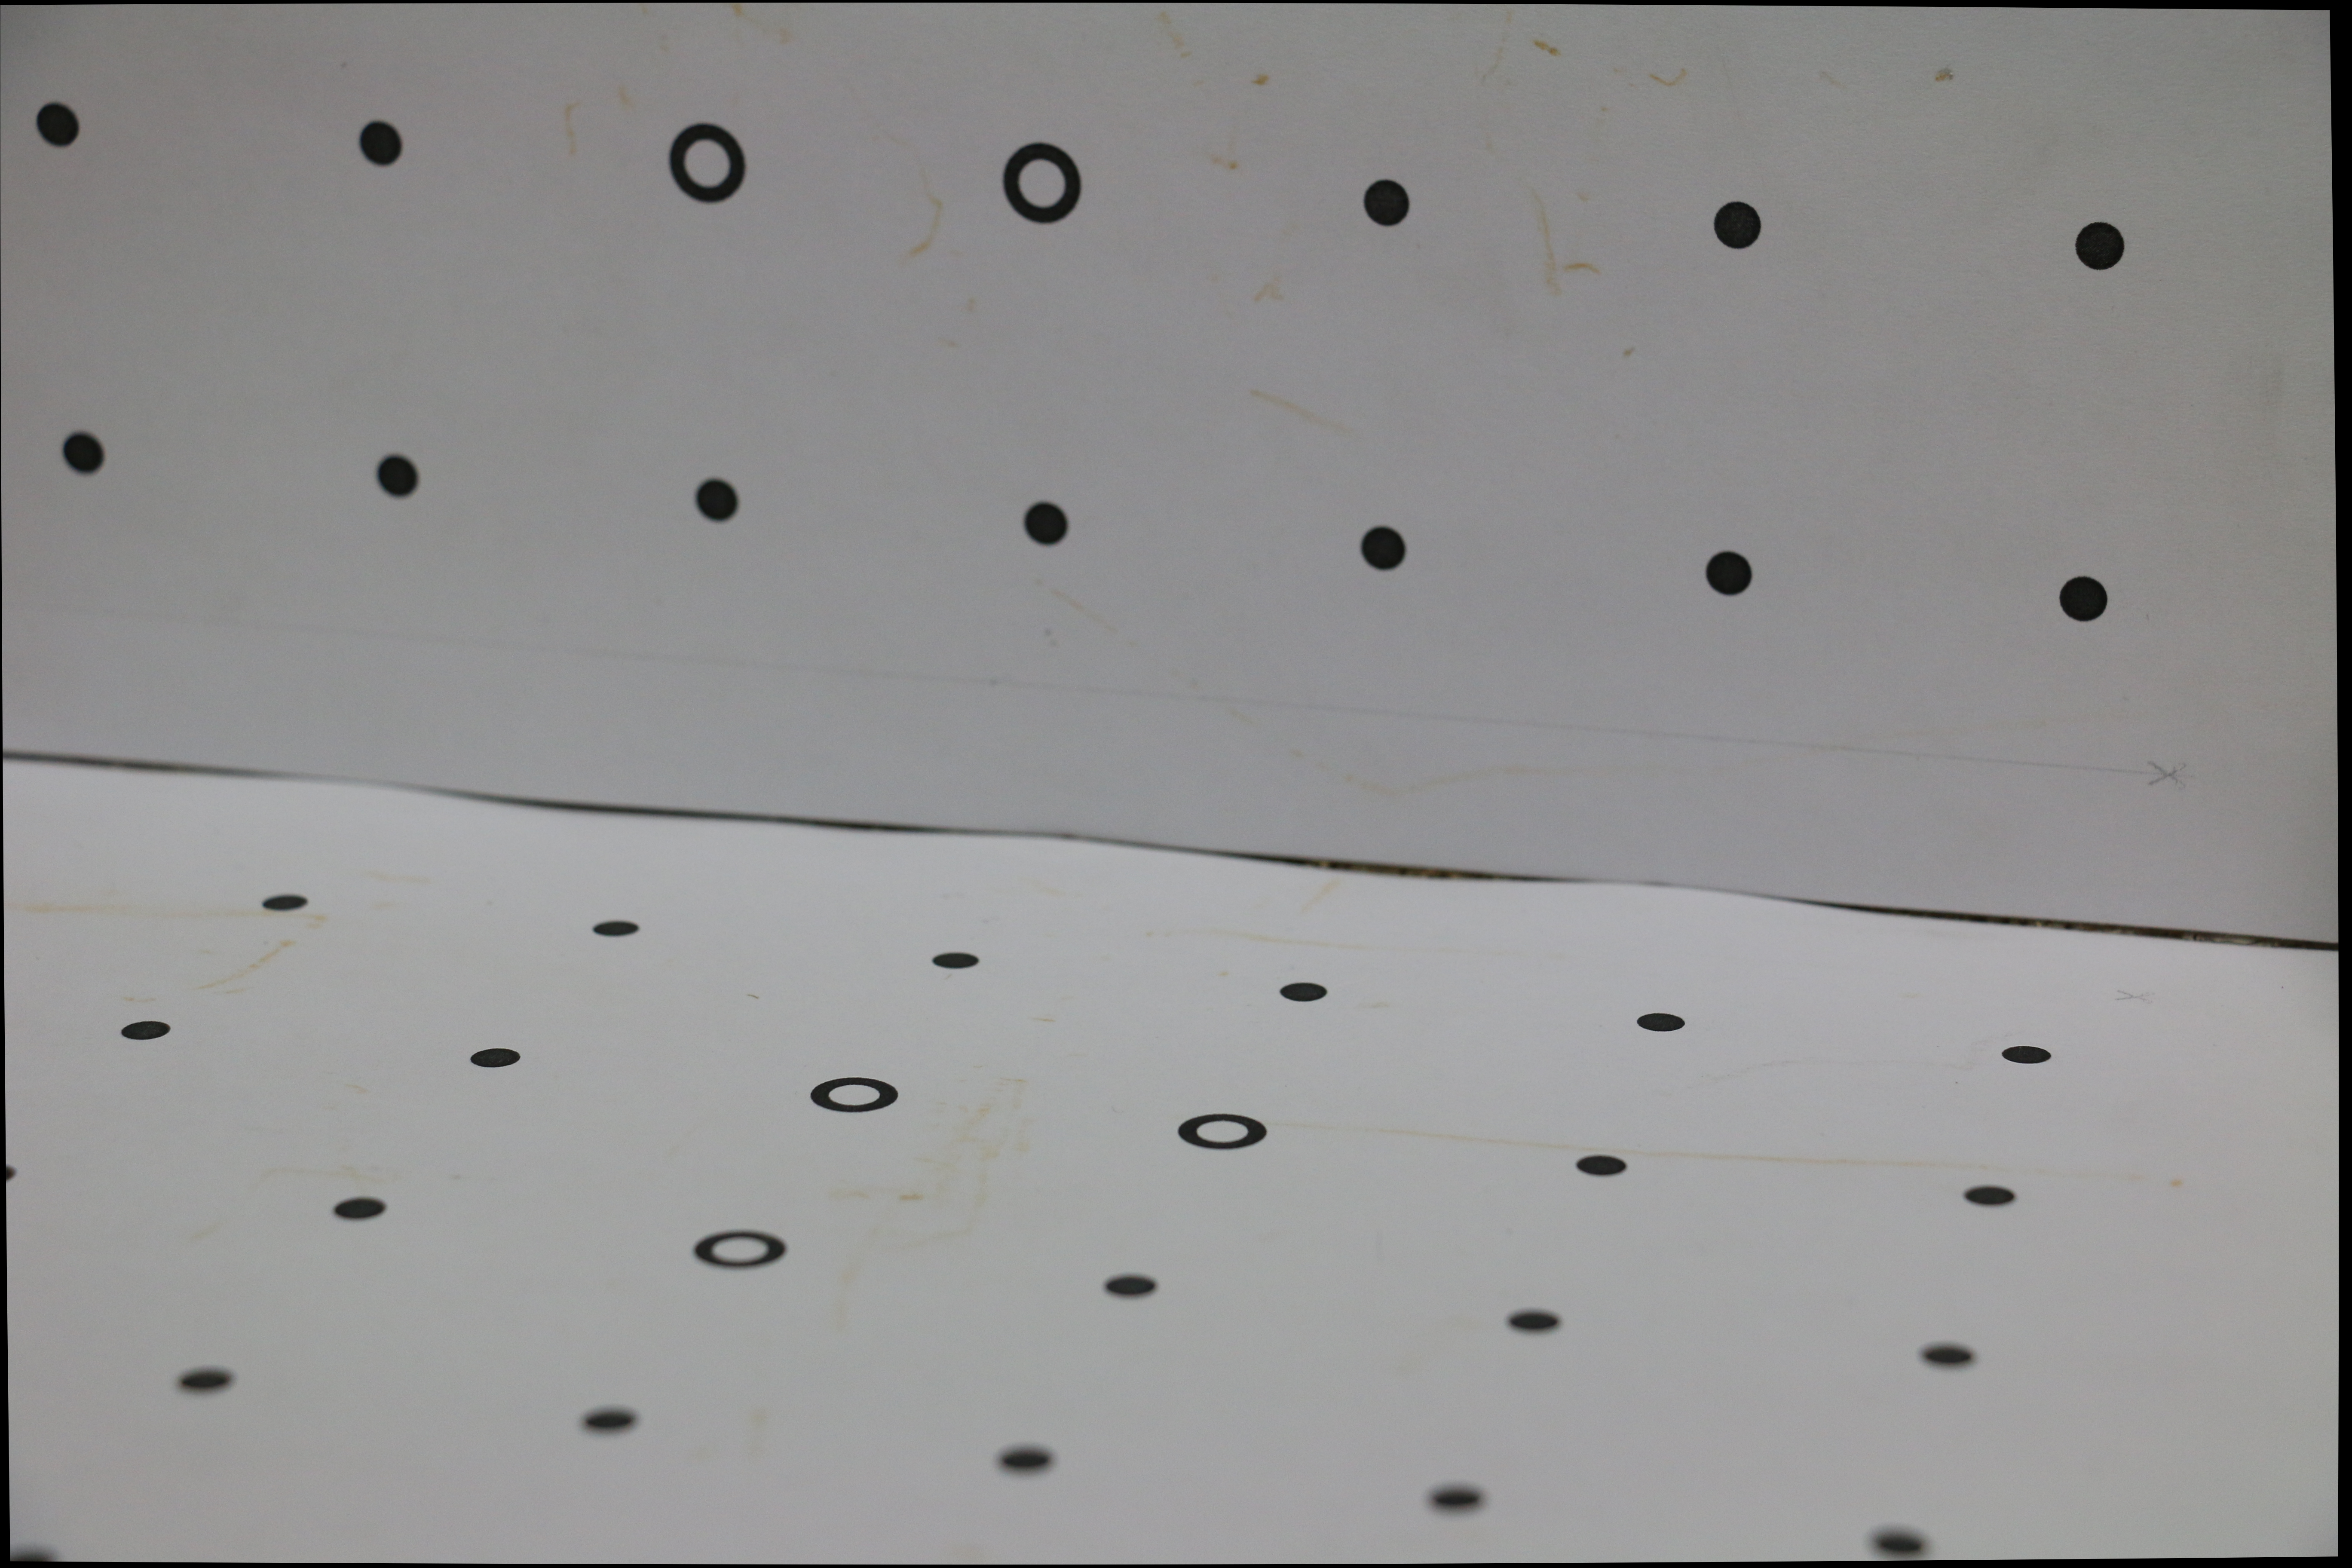
\includegraphics[scale=0.05]{undistorted} 
      \caption{Undistorted image}
      \end{figure}
 \subsection*{DLT}
 
   \begin{align*}
  \text{Calibration matrix}
  &:
  \begin{pmatrix}
  12768 & -131.677 & 3283.4 \\
  0 & 12653.8 & 2589.14 \\
  0 & 0 & 1 \\
  \end{pmatrix}\\
  \text{Rotation matrix}
  &:
  \begin{pmatrix}
   -0.9816 & 0.0143 & 0.1902 \\
   -0.0875 & -0.9199 & -0.3820 \\
   0.1965 & -0.3916 & 0.9043 \\
  \end{pmatrix}\\
  \text{Camera center}
  &:
  \begin{pmatrix}
   -0.1458\\
   -0.0653\\
   -3.04\times10^{-5}\\
  \end{pmatrix}\\
  \text{Average reprojection error}
  &: 318.676\\
  \end{align*}
 
 \subsection*{DLT with RANSAC}
   \begin{align*}
  \text{Calibration matrix}
  &:
  \begin{pmatrix}
  12668 & -31.677 & 3000.4 \\
  0 & 12633.8 & 2386.14 \\
  0 & 0 & 1 \\
  \end{pmatrix}\\
  \text{Rotation matrix}
  &:
  \begin{pmatrix}
   -0.9776 & 0.0162 & 0.1928 \\
   -0.0834 & -0.9171 & -0.3811 \\
   0.1915 & -0.3626 & 0.9123 \\
  \end{pmatrix}\\
  \text{Camera center}
  &:
  \begin{pmatrix}
   -0.1248\\
   -0.0723
   -3.64\times10^{-5}\\
  \end{pmatrix}\\
  \text{Average reprojection error}
  &: 503.276\\
  \text{Reprojection error threshold}&: 200\\
  \text{Inlier ratio threshold}&: 0.7\\
  \end{align*}
 
 \section{Wireframe overlay}
 
 \subsection*{DLT}
      \begin{figure}[H]
      \centering
      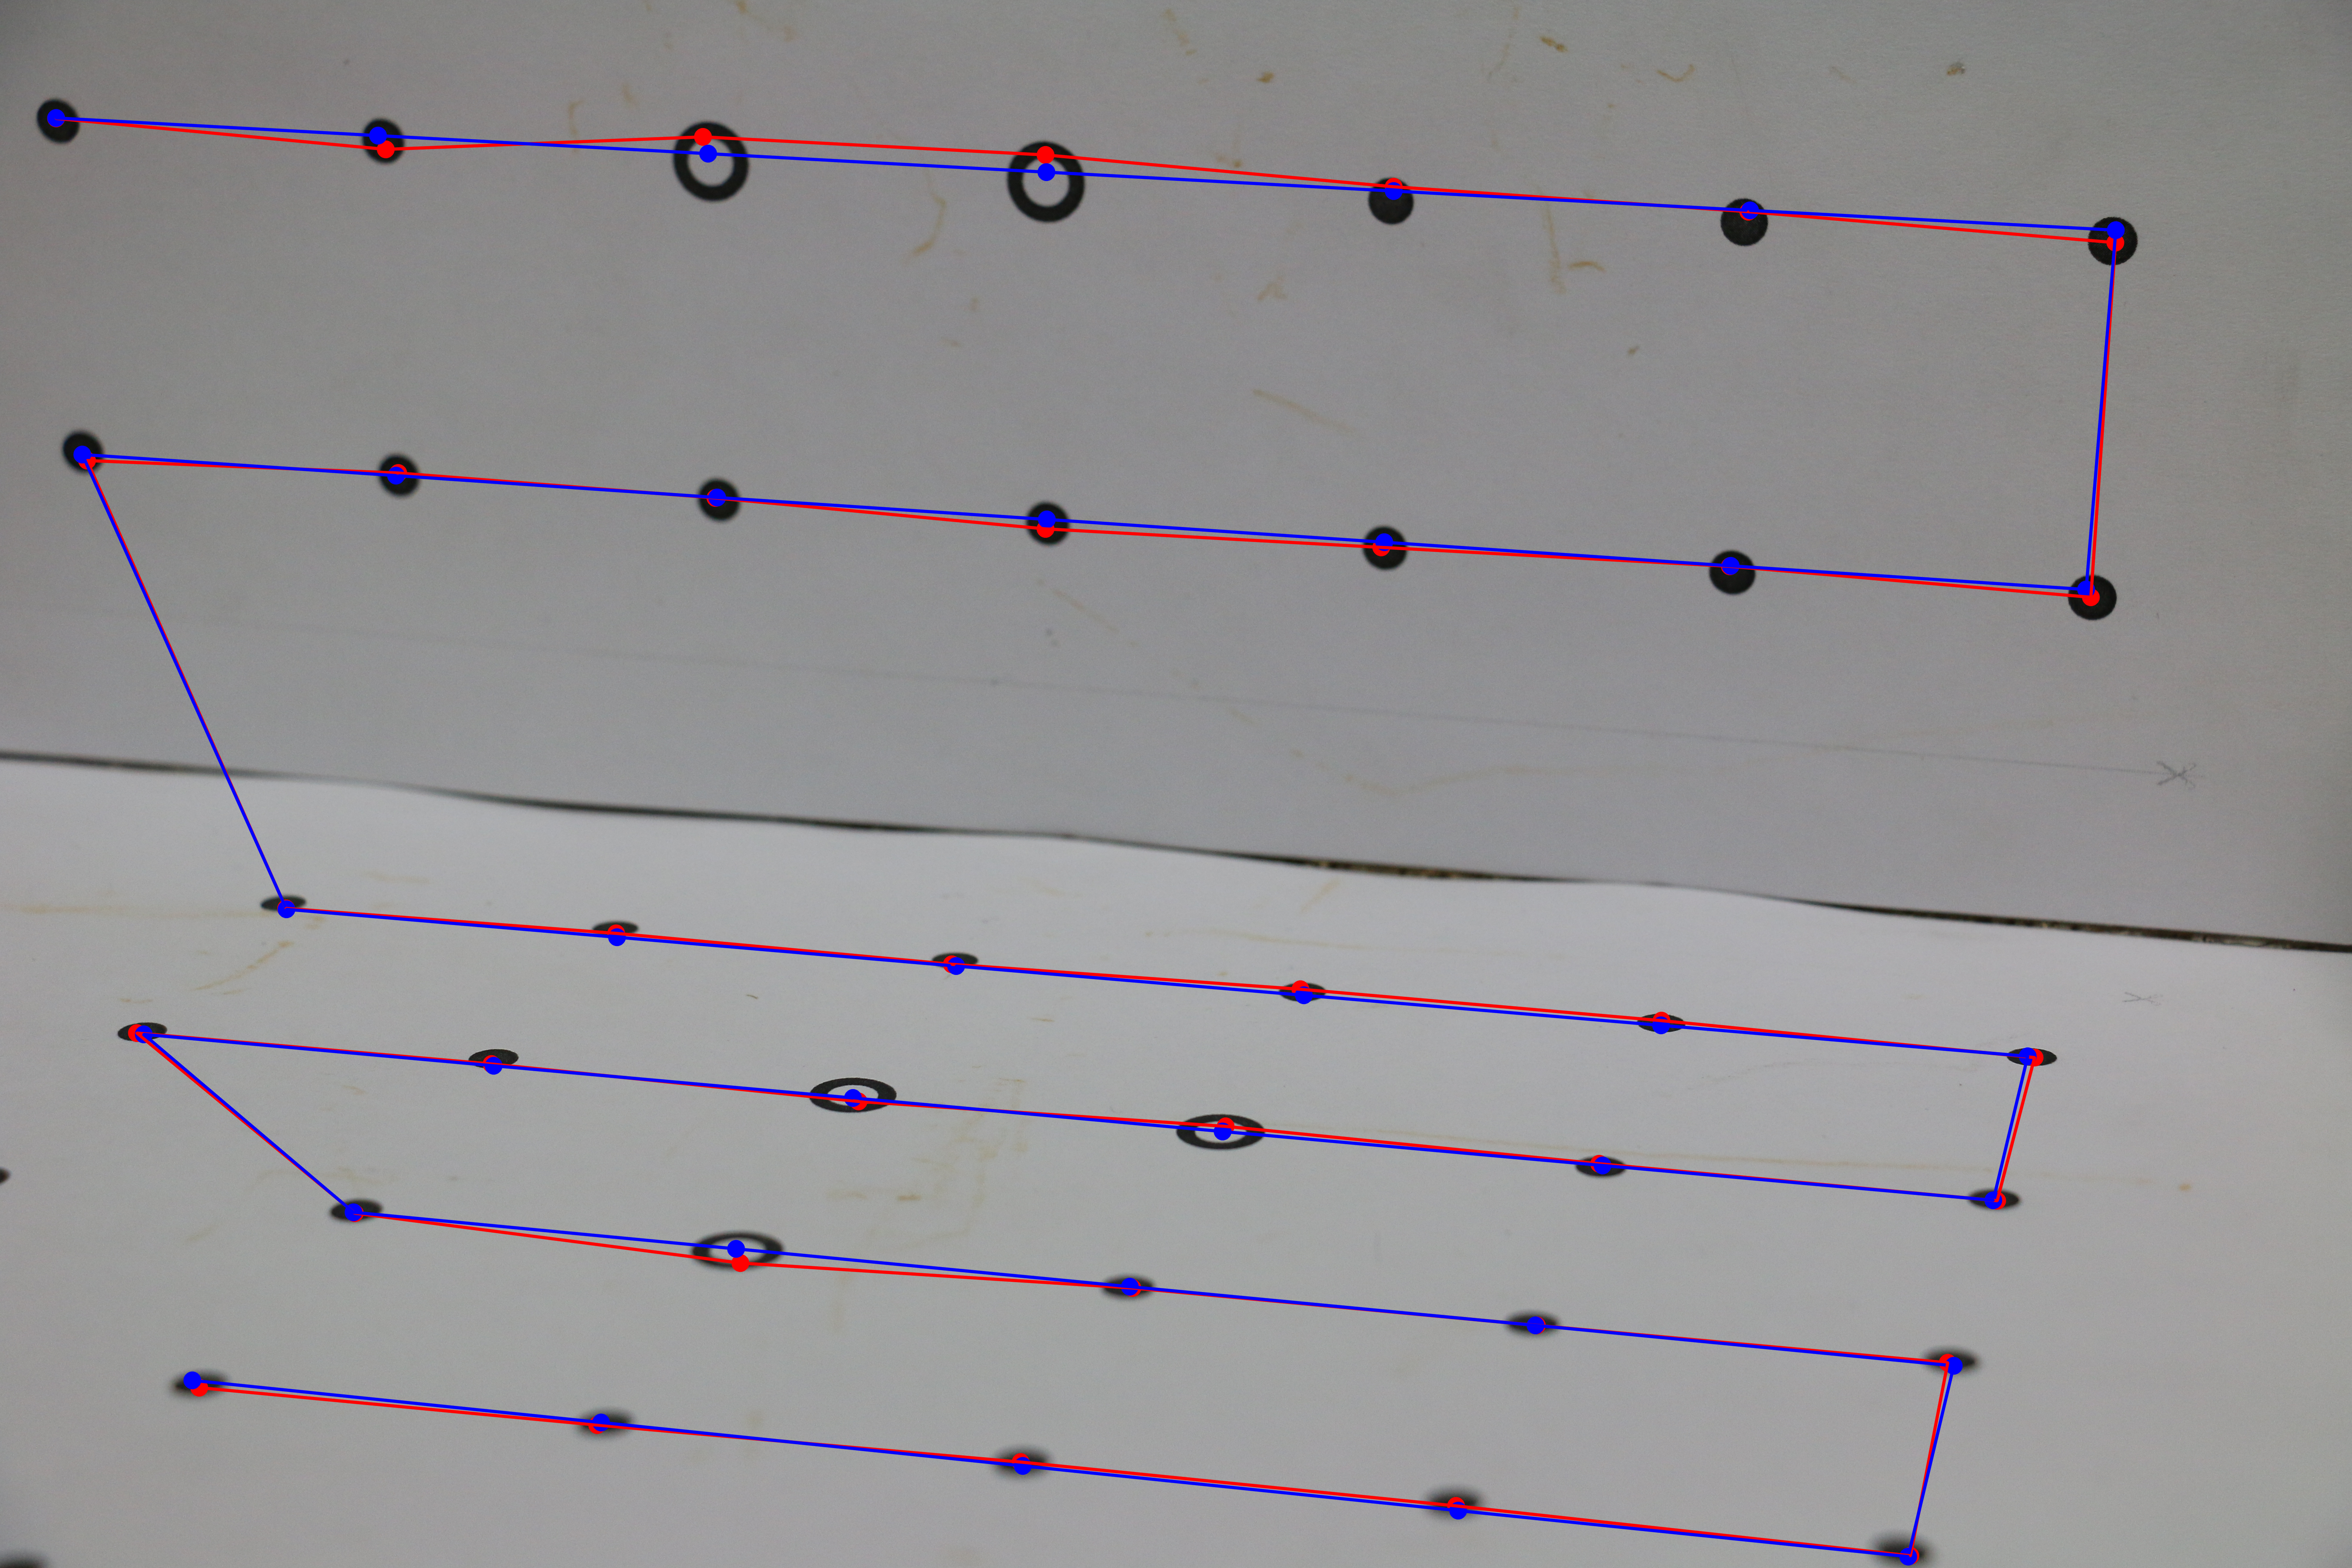
\includegraphics[scale=0.05]{grid-overlay}
      \caption{Wireframe overlayed over the 3D object after DLT calibration. Blue indicates the estimated points, red indicates the measured points.}
      
    \end{figure}
    
    \subsection*{DLT with RANSAC}
    \begin{figure}[H]
      \centering
      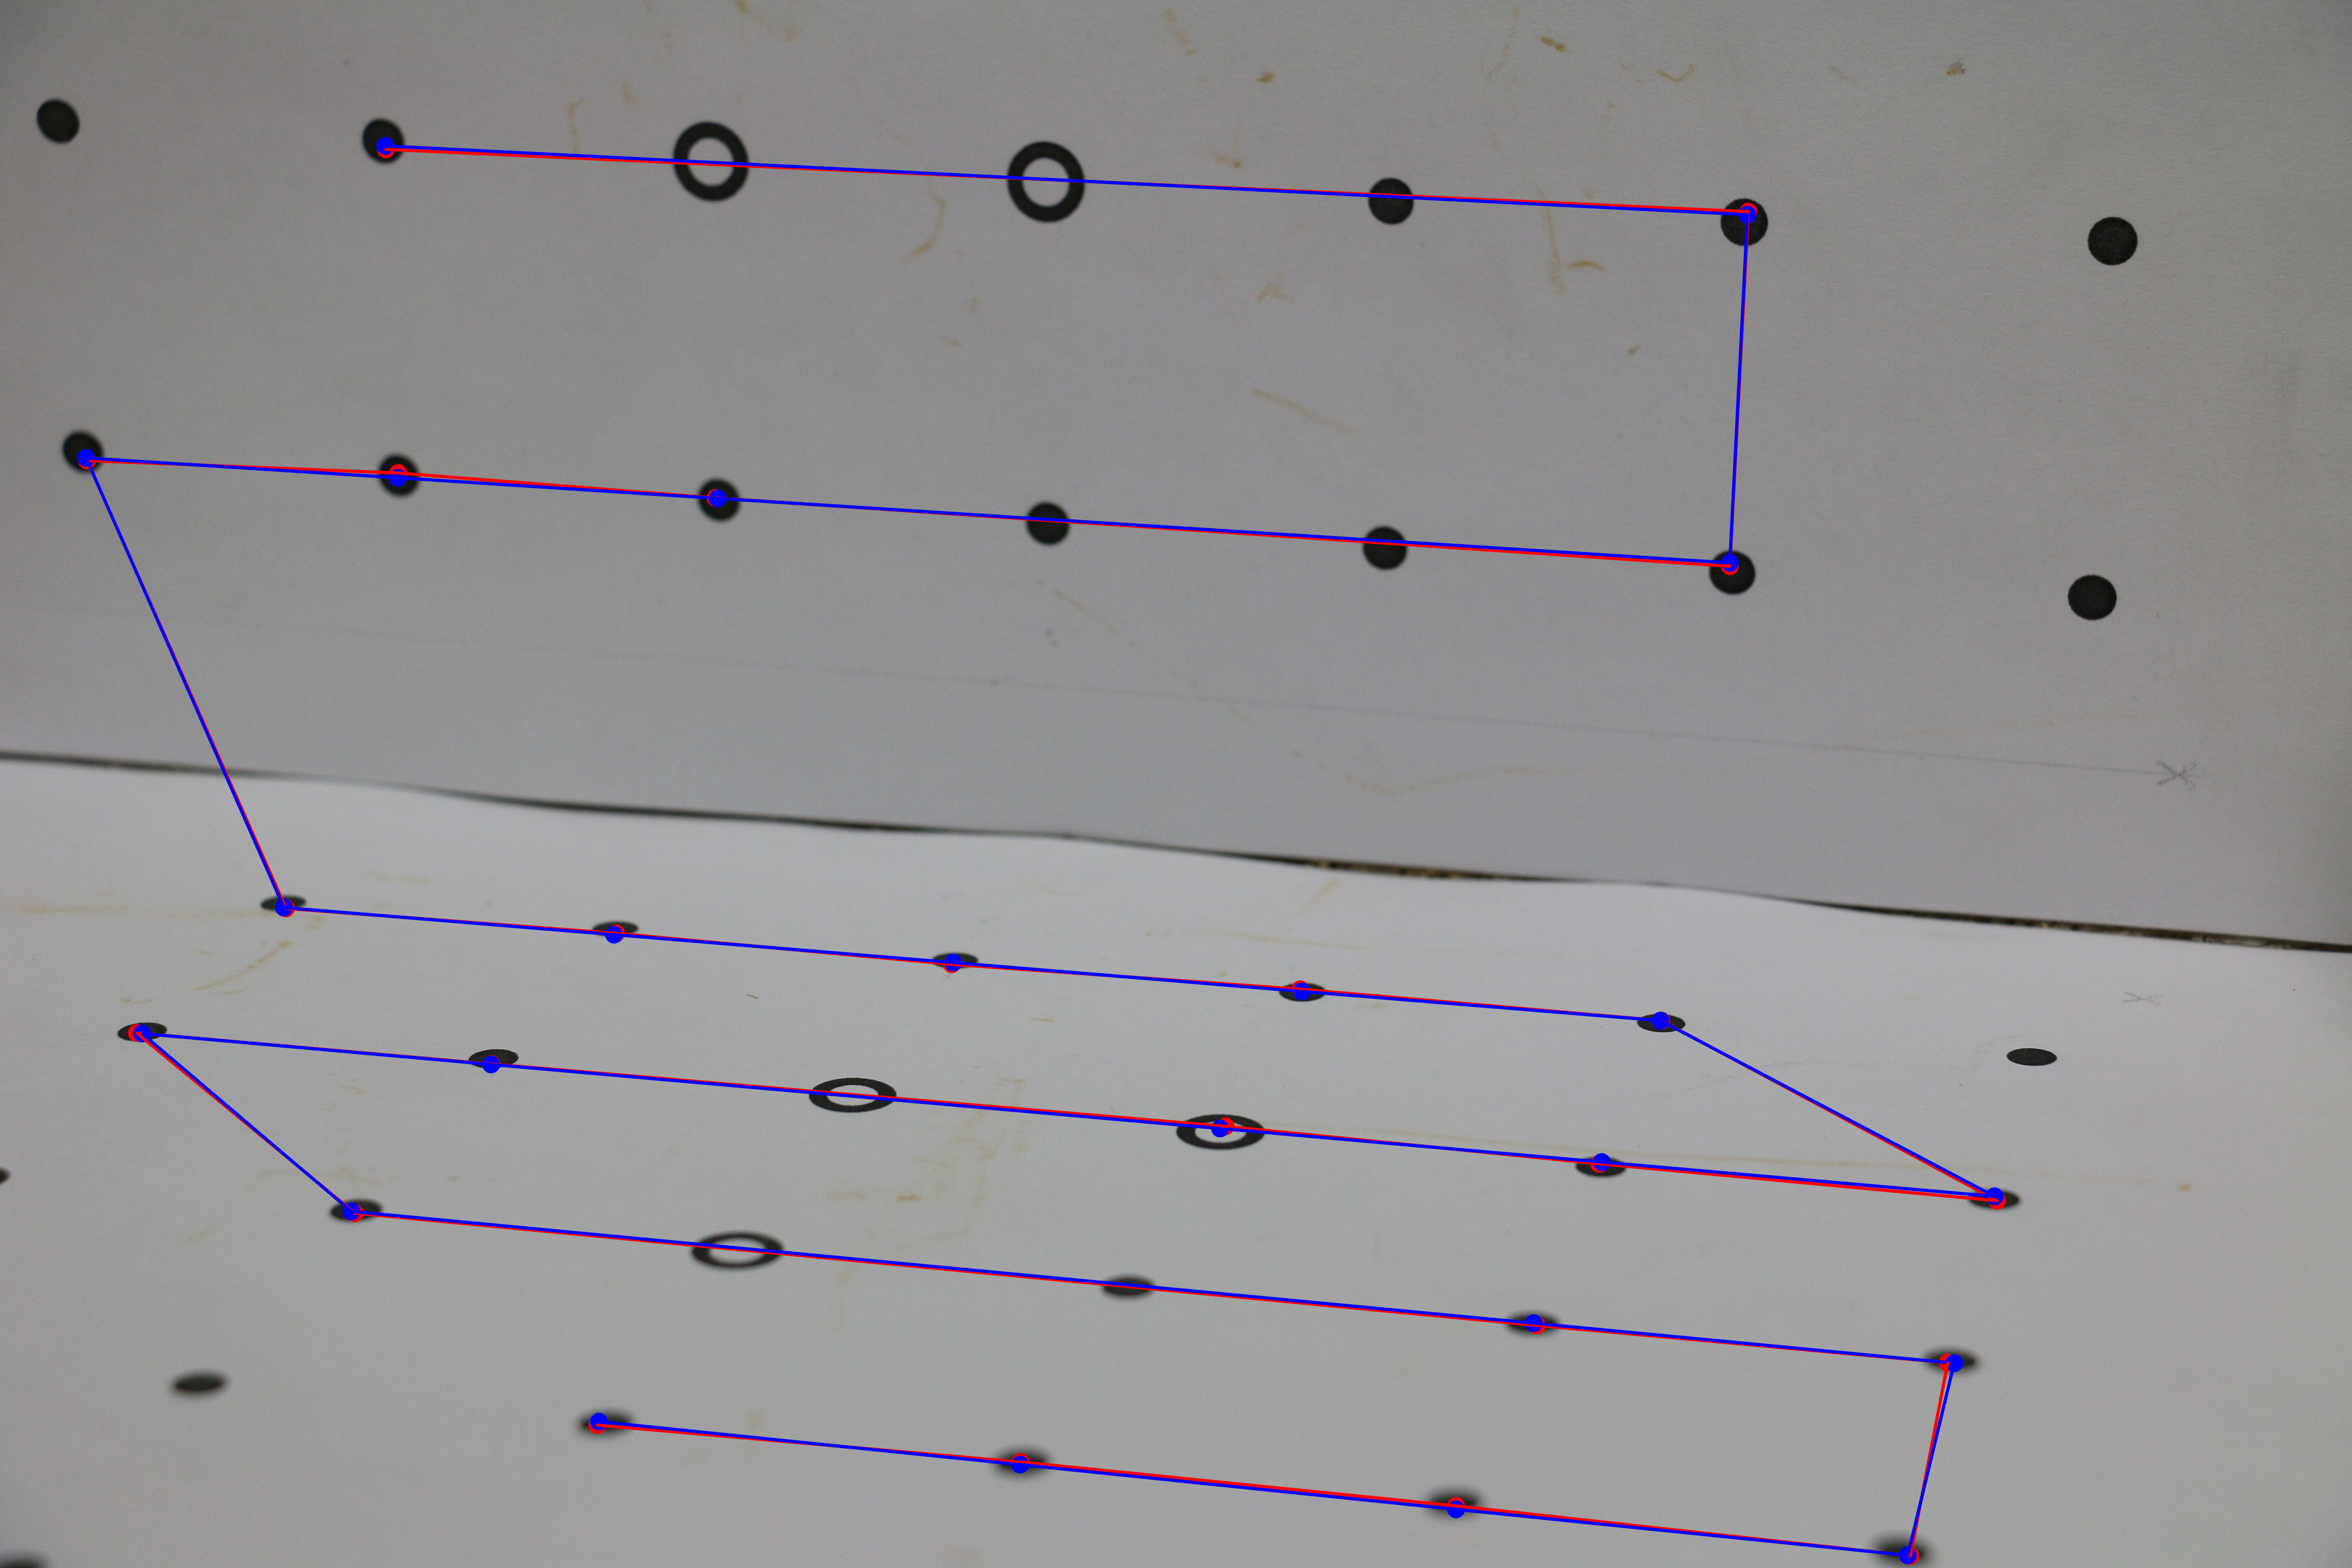
\includegraphics[scale=0.05]{grid-ransac}
      \caption{Wireframe of only the inlier points overlayed over the 3D object after DLT - RANSAC calibration. Blue indicates the estimated points, red indicates the measured points.}
      \end{figure}
    
 \section{Zhang's method}
 
 Zhang's method was tested on the provided checkerboard images using Matlab's implementation, available in the Computer Vision toolbox. Code is provided in Listing 6. The following are the estimated values:
 
     \begin{align*}
     \text{Calibration matrix}&:
     \begin{pmatrix}
       13459 & 78 & 2983\\
       0 & 13507 & 1849\\
       0 & 0 & 1\\
     \end{pmatrix}\\
     \text{Average reprojection error}
     &: 1.6417\\
     \end{align*}
     
 The results are obviously much better than the ones obtained using my implementation of DLT. One can observe that the $c_x,c_y$ values almost exactly overlap with the center of the image. The reprojection error is also less than 2 pixels.
     
 \section{Wireframe overlay using Zhang's}
 
     \begin{figure}[H]
      \centering
      \includegraphics[scale=0.2]{checkerboard-overlay}
      \caption{Wireframe overlayed over the checkerboard after calibration. Blue indicates the estimated points, red indicates the measured points.}
    \end{figure}
    
 \section{Image of world origin}
 The world origin when multiplied by the camera matrix gets projected onto the corresponding location in the image as expected.
  \begin{figure}[H]
  \centering
  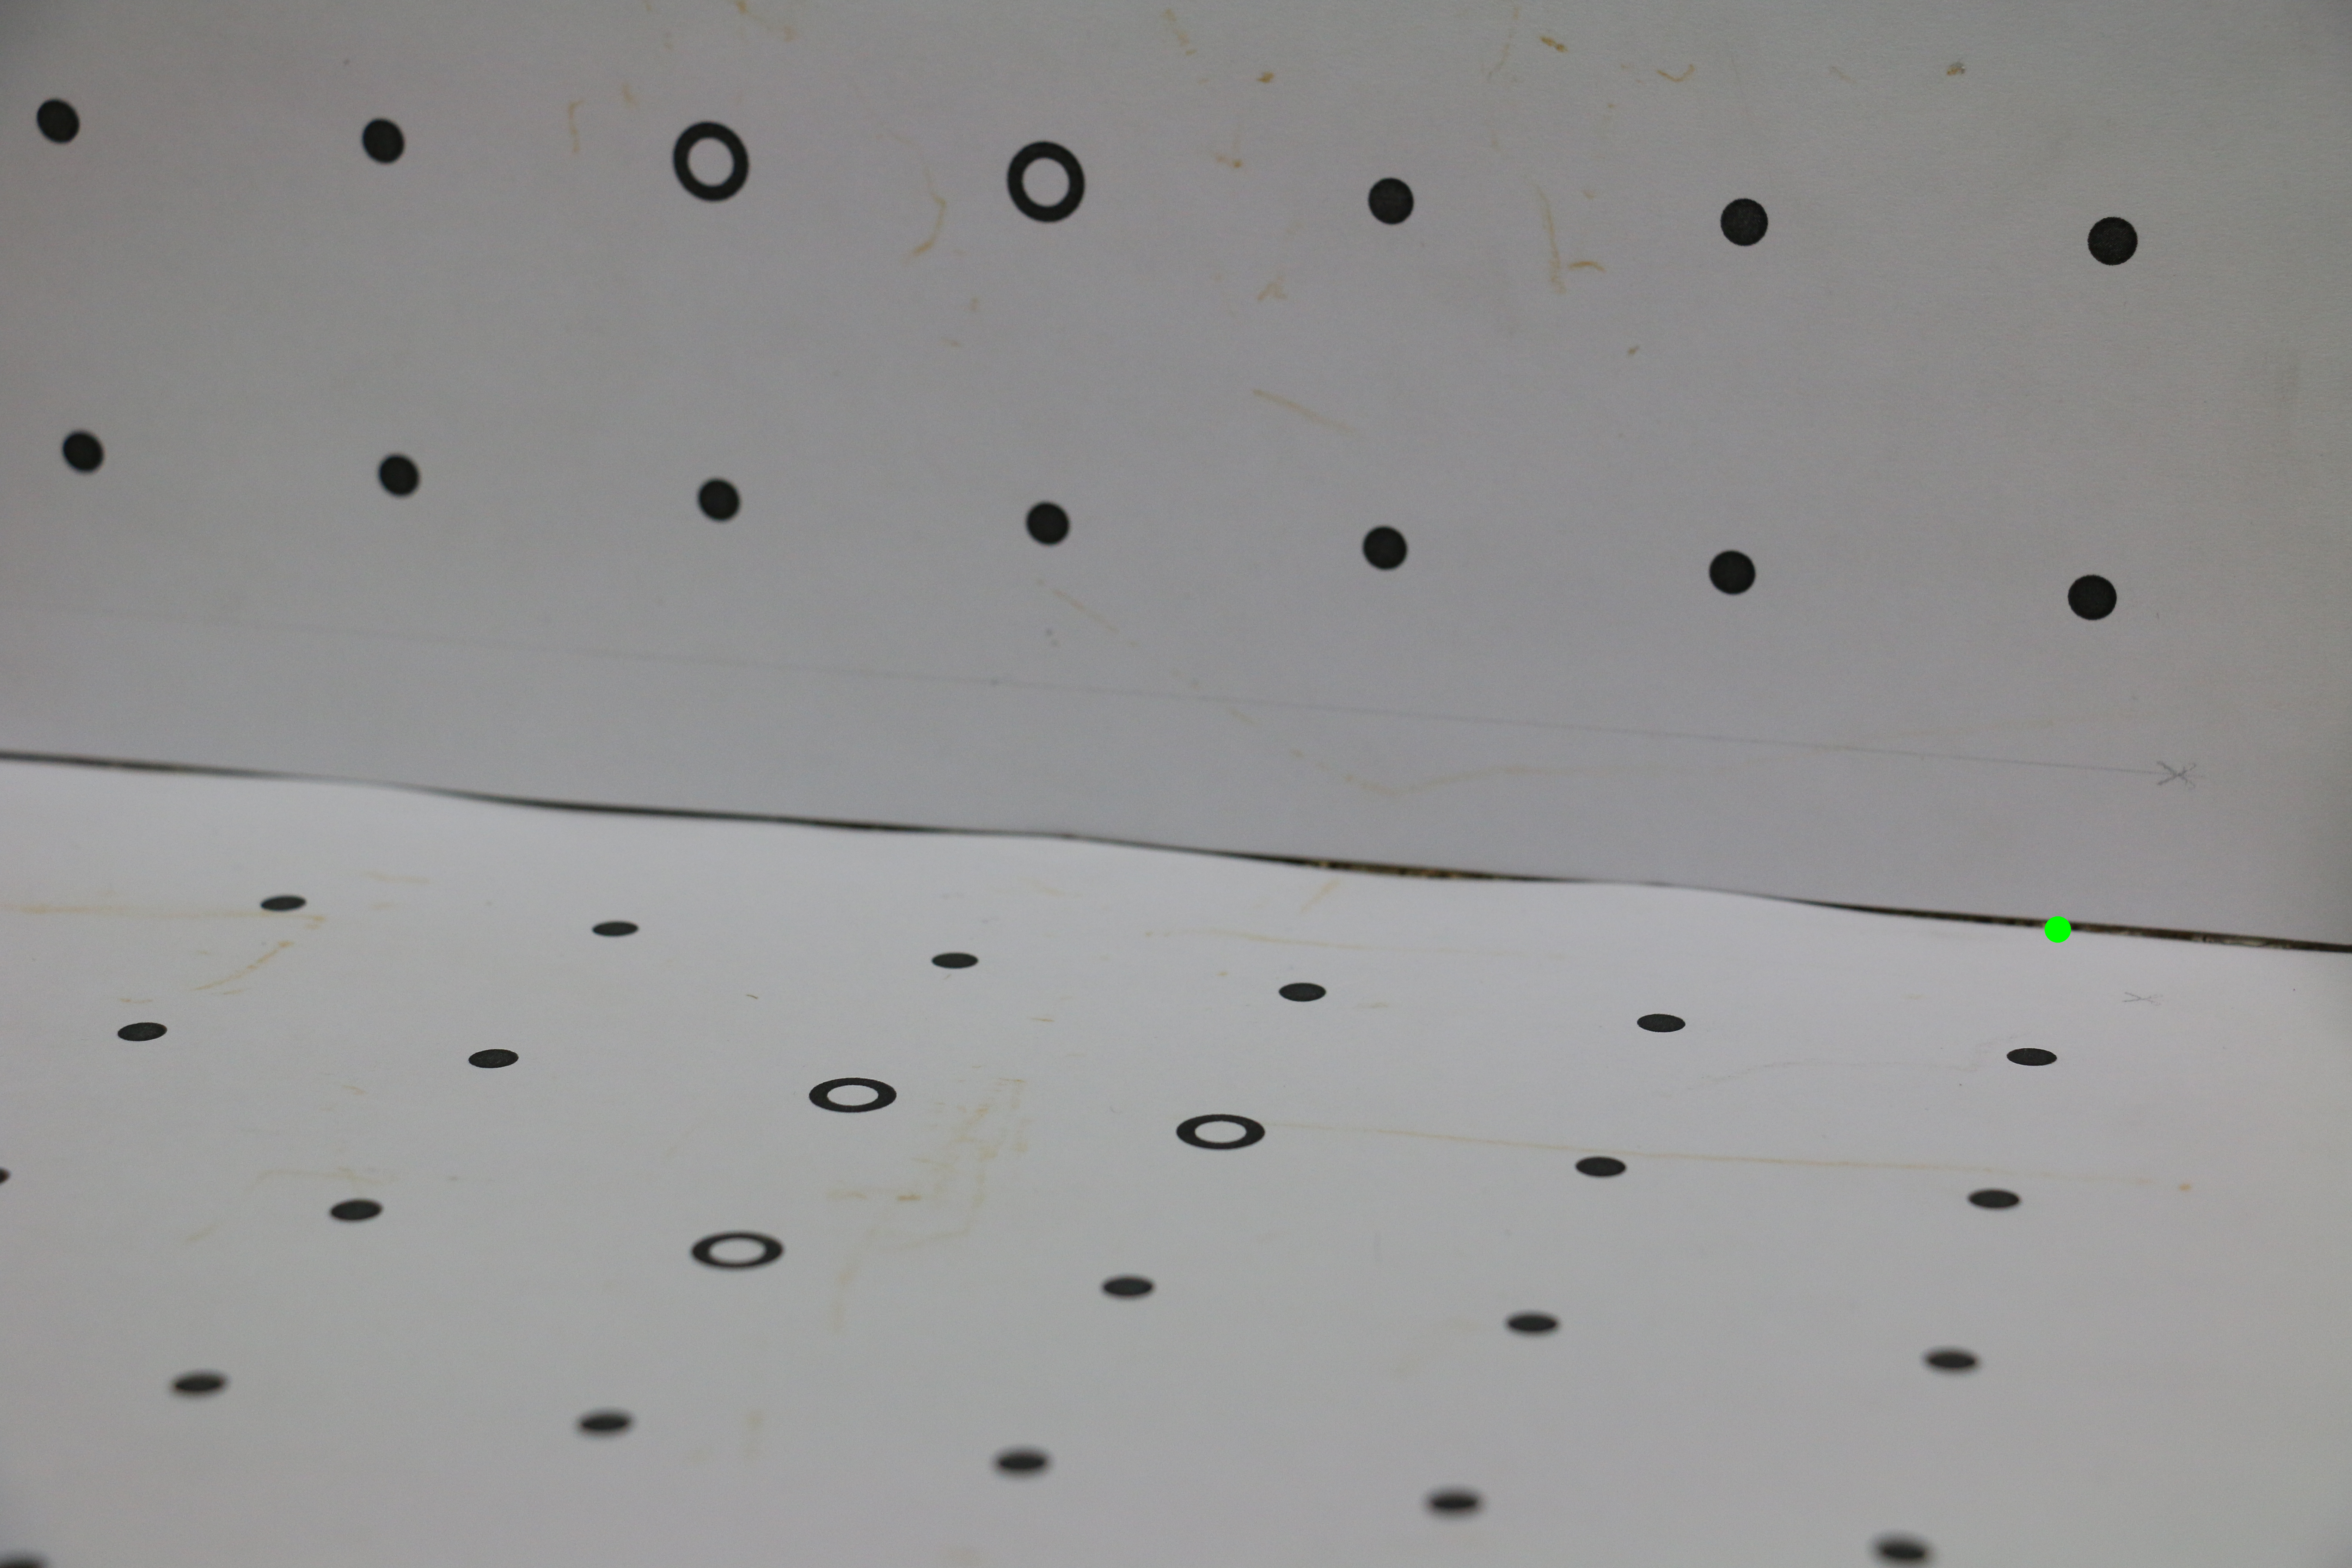
\includegraphics[scale=0.04]{origin-overlay}
  \caption{Image of the world origin}
 \end{figure}
 \section{Own setup}
  For testing the code on my setup, I used my phone camera after fixing its focal length. I used a Rubik's cube as my calibration object since it is of known dimensions and the points are easy to measure. For Zhang's method I printed out a $12 X 7$ checkerboard and took multiple images of it from different positions.
  
  \begin{figure}[H]
   \centering
   \includegraphics[scale=0.05]{cube.jpg}
   \caption{Calibration object for DLT, captured with phone camera.}
  \end{figure}
  
  \begin{figure}[H]
   \centering
   \includegraphics[scale=0.08]{checkerboard-phone}
   \caption{Calibration object for Zhang's, captured with phone camera.}
  \end{figure}

  \section{Results using own setup}
    \subsection*{DLT}
    \begin{align*}
     \text{Calibration matrix}
     &: 
     \begin{pmatrix}
       -4209.56 & 22.7655 & 1331.44\\
       0 & -4186.34 & 2174.04\\
       0 & 0 & 1\\
     \end{pmatrix}\\
     \text{Rotation matrix}
     &:
     \begin{pmatrix}
      -0.7607 & -0.0113 & 0.6489 \\
      0.4814 & -0.6802 & 0.5526 \\
      0.4351 & 0.7329 & 0.5229 \\
     \end{pmatrix}\\
      \text{Camera center}
      &:
      \begin{pmatrix}
      0.0311\\
      0.0550\\
      3.0356\times10^{-5}\\
      \end{pmatrix}\\
     \text{Average reprojection error}
     &: 86.6504
    \end{align*}
     
     \begin{figure}[H]
      \centering
      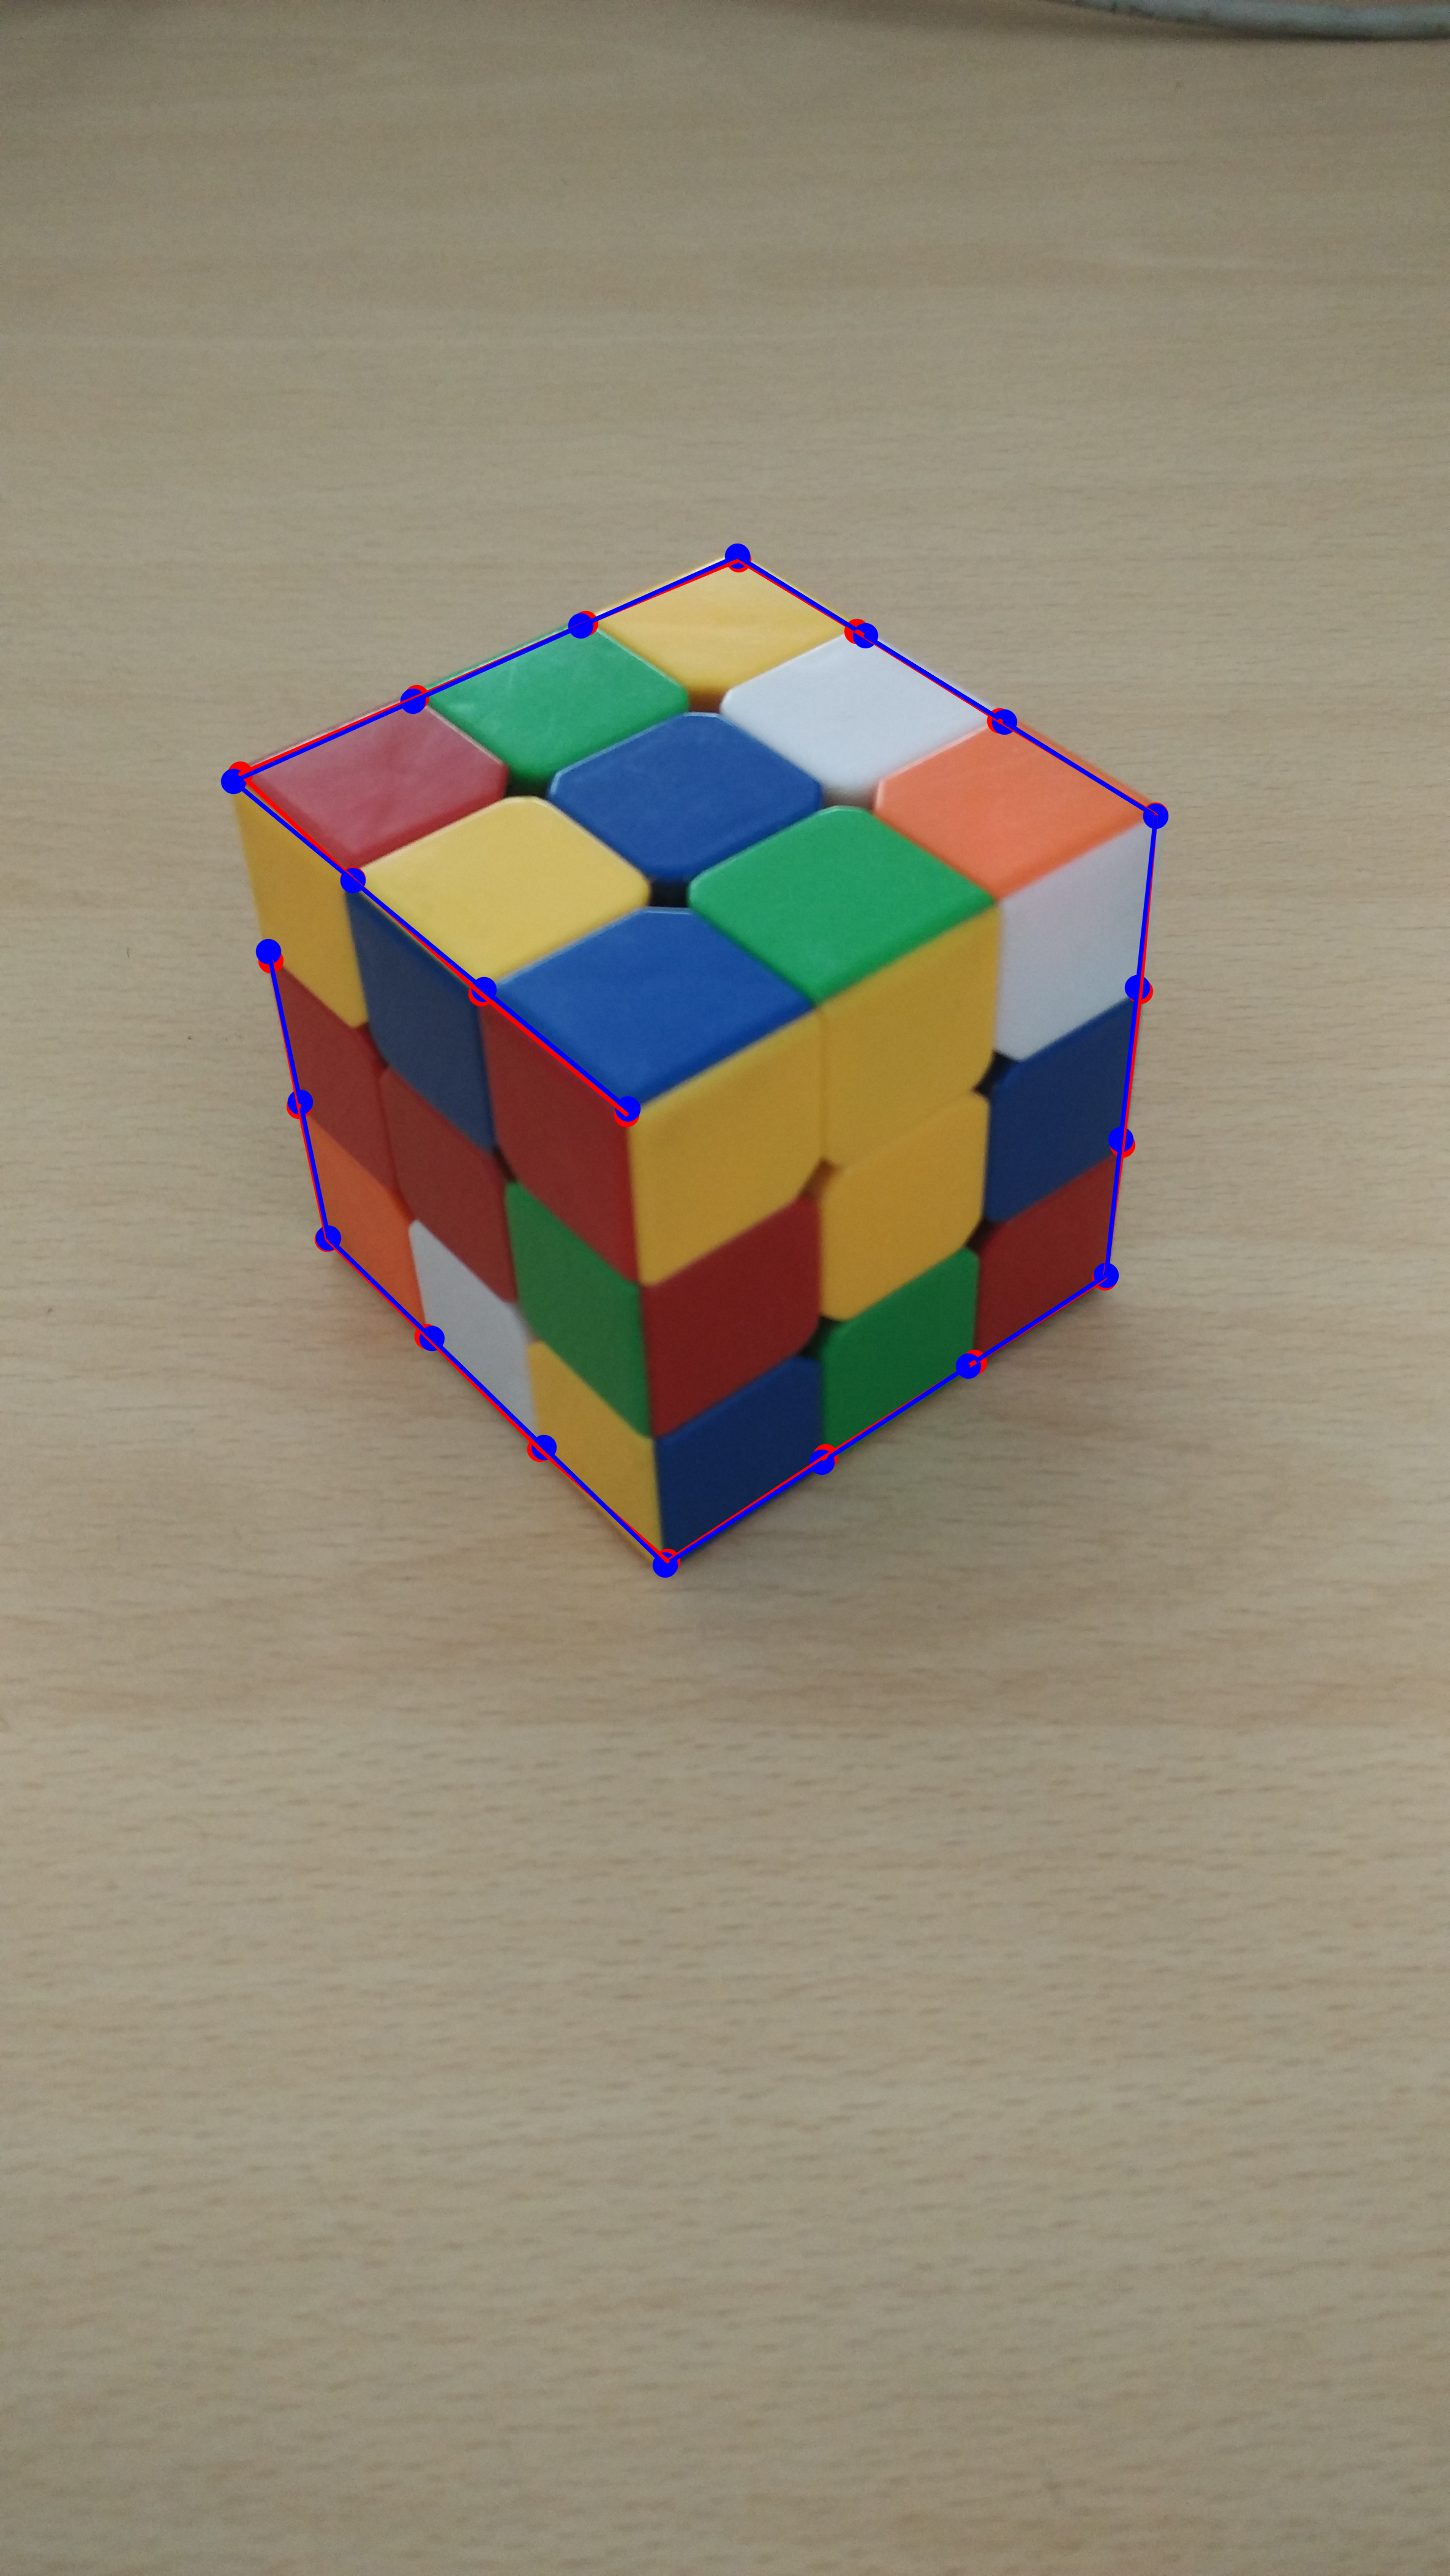
\includegraphics[scale=0.06]{cube-overlay}
      \caption{Wireframe overlayed over the cube object after calibration. Blue indicates projected points, red indicates measured points.}
     \end{figure}
    
    \subsection*{DLT with RANSAC}
    
     \begin{align*}
     \text{Calibration matrix}
     &: 
     \begin{pmatrix}
       -4342.95 & -24.8555 & 911.788\\
       0 & -4377.99 & 1868.58\\
       0 & 0 & 1\\
     \end{pmatrix}\\
     \text{Rotation matrix}
     &:
     \begin{pmatrix}
      -0.8037 & -0.0652 & 0.5864 \\
      0.4369 & -0.7340 & 0.5199 \\
      0.3964 & 0.676 & 0.6211 \\
     \end{pmatrix}\\
      \text{Camera center}
      &:
      \begin{pmatrix}
      0.0319\\
      0.0564\\
      3.1294\times10^{-5}\\
      \end{pmatrix}\\
     \text{Average reprojection error}
     &: 198.293\\
     \text{Reprojection error threshold}&: 50\\
     \text{Inlier ratio threshold}&: 0.5\\
    \end{align*}
    
     \begin{figure}[H]
      \centering
      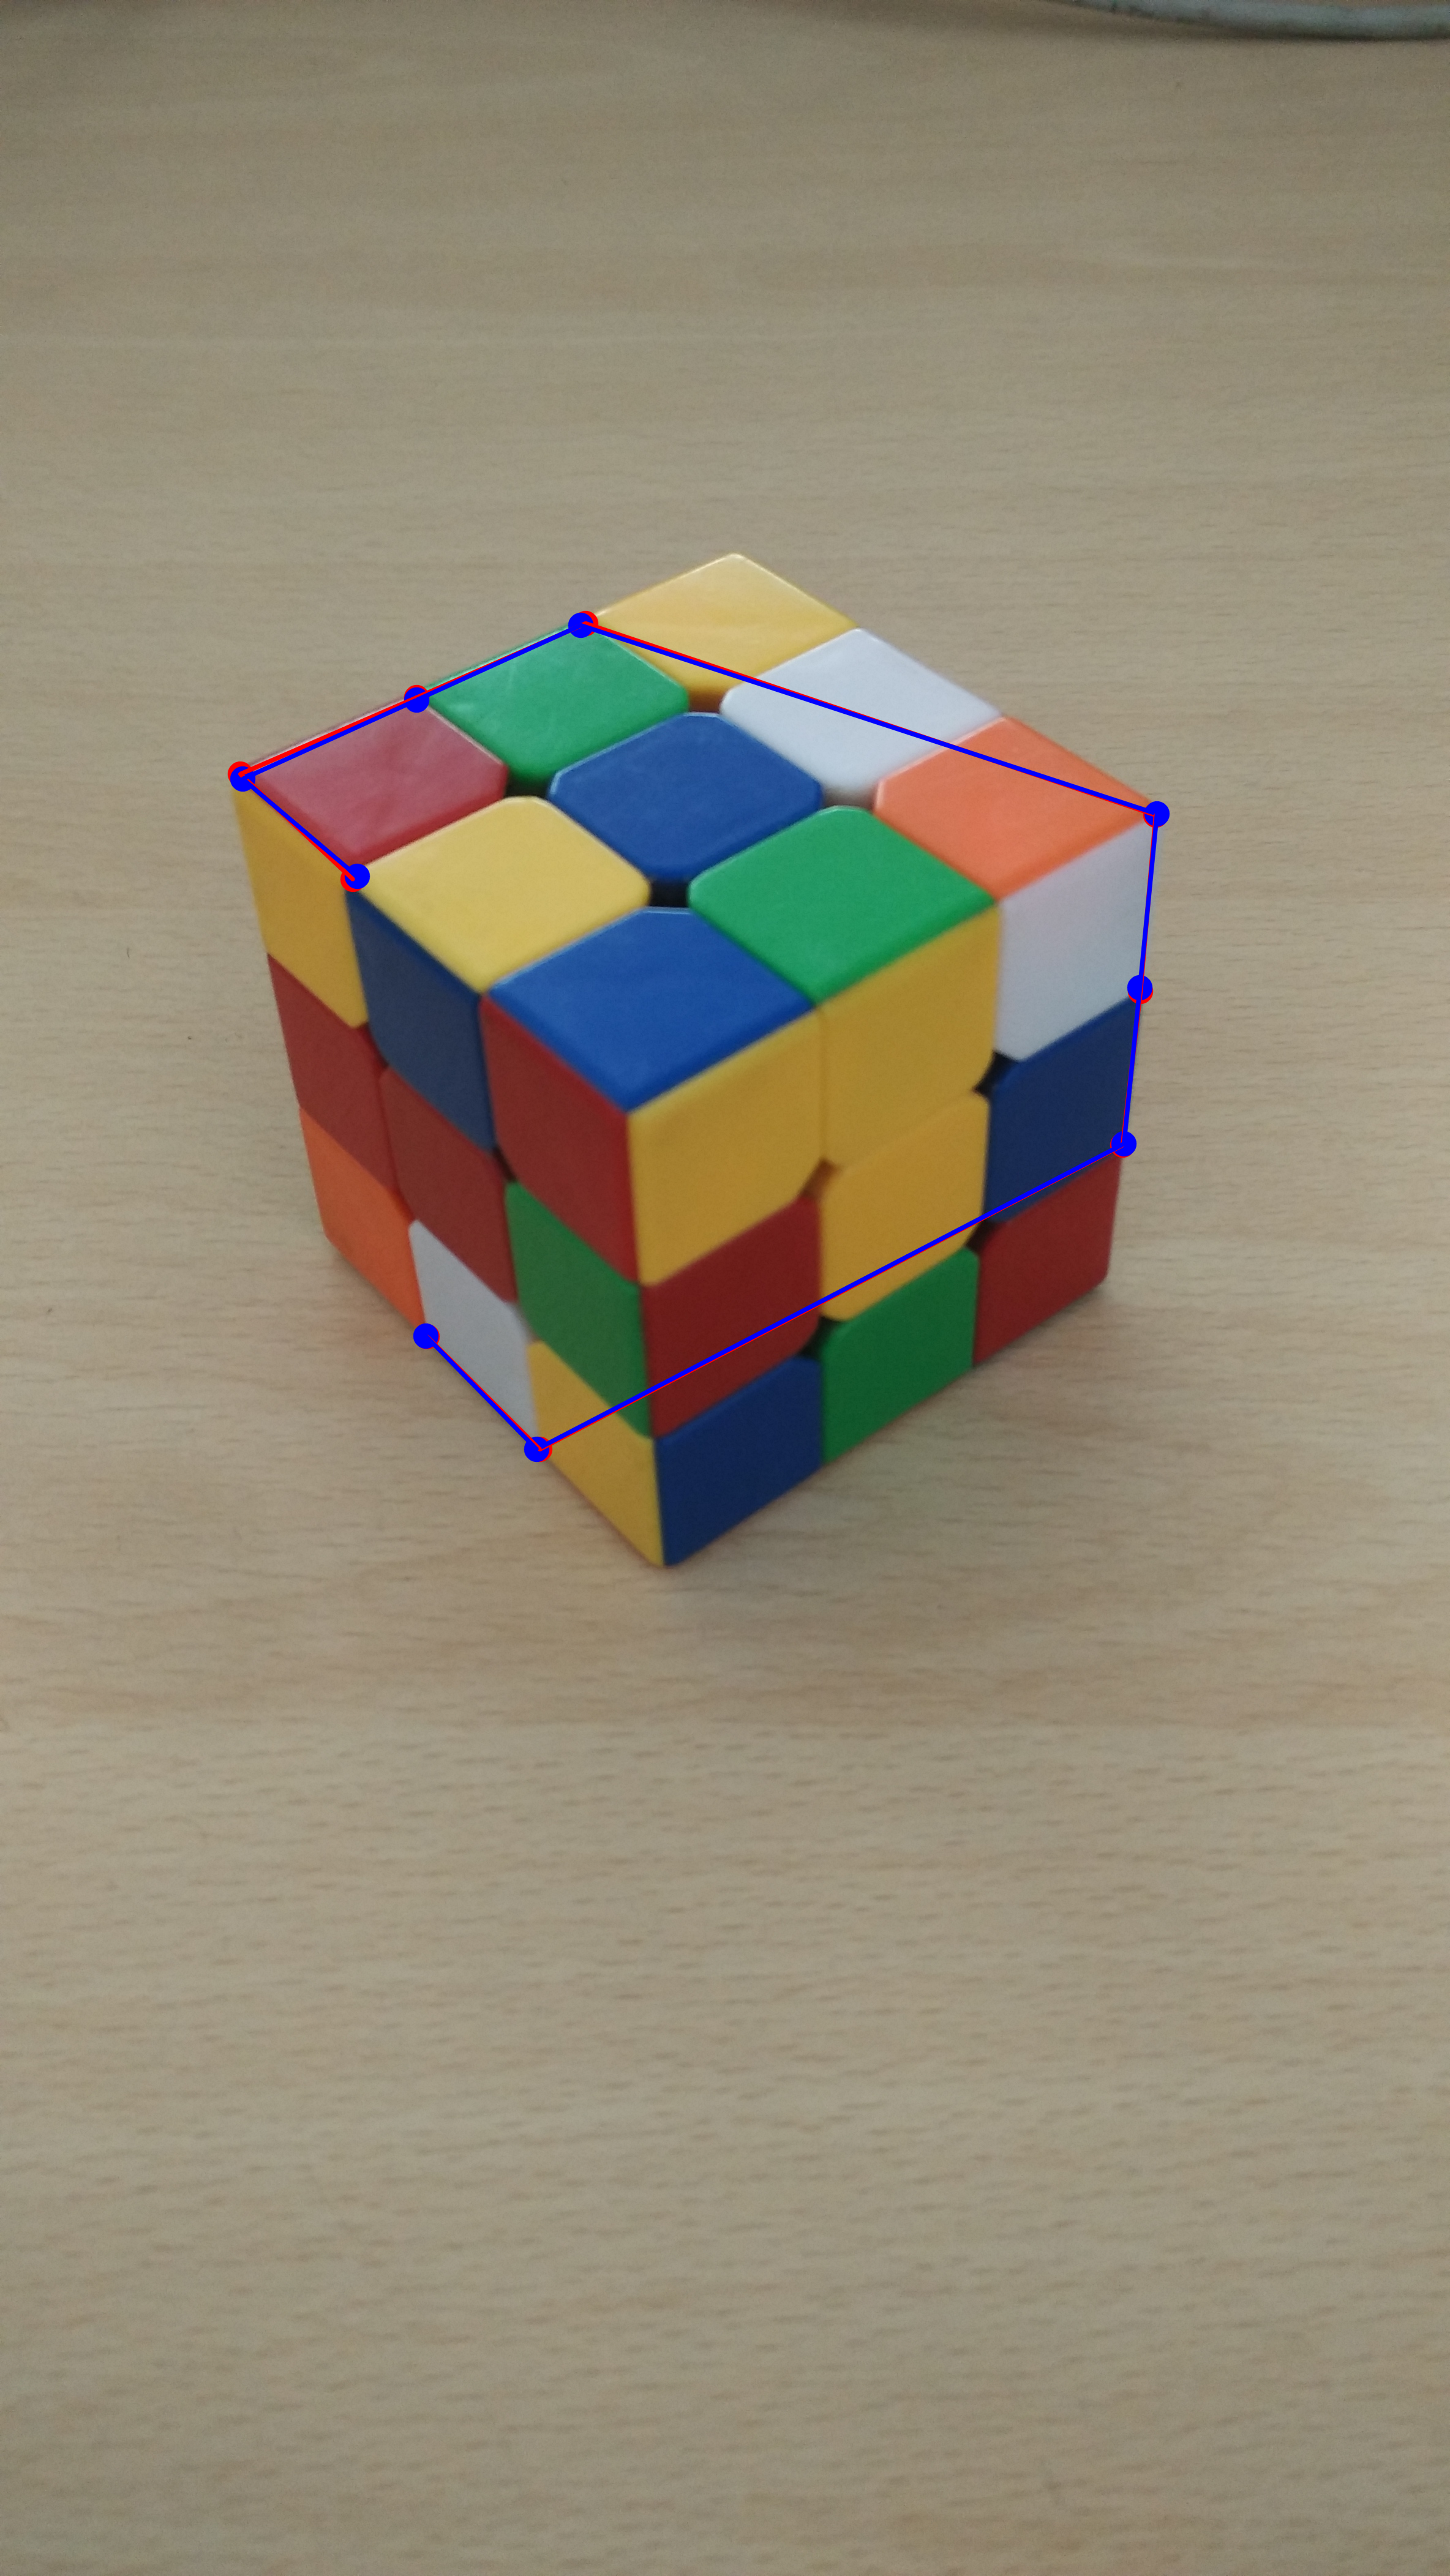
\includegraphics[scale=0.06]{cube-ransac}
      \caption{Wireframe of only the inlier points overlayed over the cube object after calibration. Blue indicates projected points, red indicates measured points.}
     \end{figure}

    \subsection*{Zhang's}
    \begin{align*}
     \text{Calibration matrix}&: 
     \begin{pmatrix}
       3765.8 & -4.1 & 2067.7 \\
       0 & 3757.1 & 1204.7 \\
       0 & 0 & 1\\
     \end{pmatrix}\\
     \text{Average reprojection error}
     &: 1.5617\\
     \end{align*}
     
    \begin{figure}[H]
      \centering
      \includegraphics[scale=0.2]{checkerboard-phone-overlay}
      \caption{Wireframe overlayed over the checkerboard after calibration. Blue indicates the estimated points, red indicates the measured points.}
    \end{figure}
    
    \section{Code}
    
    All the code files can be found \href{https://drive.google.com/drive/folders/1aRjtnyrv5AyIaVY0OsNKUHnJqoDyX3oz?usp=sharing}{here}. The main algorithms are implemented in Listing 2.
    
    \lstinputlisting[language=C++, caption=calibrator.hpp]{../src/calibrator.hpp}
    \lstinputlisting[language=C++, caption=calibrator.cpp]{../src/calibrator.cpp}
    \lstinputlisting[language=C++, caption=run\_dlt.cpp]{../src/run_dlt.cpp}
    \lstinputlisting[language=C++, caption=run\_ransac\_dlt.cpp]{../src/run_ransac_dlt.cpp}
    \lstinputlisting[language=make, caption=CMakeLists.txt]{../CMakeLists.txt}
    \lstinputlisting[language=Matlab,caption=run\_zhangs.m]{../matlab/run_zhangs.m}
\end{document}
